%
% Main document
% ===========================================================================
% This is part of the document "Project documentation template".
% Authors: brd3
%

%---------------------------------------------------------------------------
\documentclass[
	a4paper,					% paper format
	10pt,							% fontsize
	twoside,					% double-sided
	openright,				% begin new chapter on right side
	notitlepage,			% use no standard title page
	parskip=half,			% set paragraph skip to half of a line
]{scrreprt}					% KOMA-script report
%---------------------------------------------------------------------------

\raggedbottom
\KOMAoptions{cleardoublepage=plain}			% Add header and footer on blank pages


% Load Standard Packages:
%---------------------------------------------------------------------------
\usepackage[standard-baselineskips]{cmbright}

\usepackage[ngerman]{babel}										% german hyphenation
%\usepackage[latin1]{inputenc}  							% Unix/Linux - load extended character set (ISO 8859-1)
\usepackage[ansinew]{inputenc}  							% Windows - load extended character set (ISO 8859-1)
\usepackage[T1]{fontenc}											% hyphenation of words with �,� and �
\usepackage{textcomp}													% additional symbols
\usepackage{ae}																% better resolution of Type1-Fonts 
\usepackage{fancyhdr}													% simple manipulation of header and footer 
\usepackage{graphicx}                      		% integration of images
\usepackage{float}														% floating objects
\usepackage{caption}													% for captions of figures and tables
\usepackage{booktabs}													% package for nicer tables
\usepackage{tocvsec2}													% provides means of controlling the sectional numbering
%---------------------------------------------------------------------------

% Load Math Packages
%---------------------------------------------------------------------------
\usepackage{amsmath}                    	   	% various features to facilitate writing math formulas
\usepackage{amsthm}                       	 	% enhanced version of latex's newtheorem
\usepackage{amsfonts}                      		% set of miscellaneous TeX fonts that augment the standard CM
\usepackage{amssymb}													% mathematical special characters
\usepackage{exscale}													% mathematical size corresponds to textsize
%---------------------------------------------------------------------------

% Package to facilitate placement of boxes at absolute positions
%---------------------------------------------------------------------------
\usepackage[absolute]{textpos}
\setlength{\TPHorizModule}{1mm}
\setlength{\TPVertModule}{1mm}
%---------------------------------------------------------------------------					
			
% Definition of Colors
%---------------------------------------------------------------------------
\RequirePackage{color}                          % Color (not xcolor!)
\definecolor{linkblue}{rgb}{0,0,0.8}            % Standard
\definecolor{darkblue}{rgb}{0,0.08,0.45}        % Dark blue
\definecolor{brickred}{cmyk}{0,0.89,0.94,0.28}  % Brickred
%\definecolor{linkcolor}{rgb}{0,0,0.8}     			% Blue for the web- and cd-version!
\definecolor{linkcolor}{rgb}{0,0,0}        			% Black for the print-version!
\definecolor{bfhred}{rgb}{0.776,0,0.066}  			% Red
%---------------------------------------------------------------------------

% Hyperref Package (Create links in a pdf)
%---------------------------------------------------------------------------
\usepackage[
	pdftex,ngerman,bookmarks,plainpages=false,pdfpagelabels,
	backref = {false},										% No index backreference
	colorlinks = {true},                  % Color links in a PDF
	hypertexnames = {true},               % no failures "same page(i)"
	bookmarksopen = {true},               % opens the bar on the left side
	bookmarksopenlevel = {0},             % depth of opened bookmarks
	pdftitle = {Projekt 2 - AI Challenge},	   	% PDF-property
	pdfauthor = {kases1, kustl1},        					  % PDF-property
	pdfsubject = {LaTeX Template},        % PDF-property
	linkcolor = {linkcolor},              % Color of Links
	citecolor = {linkcolor},              % Color of Cite-Links
	urlcolor = {linkcolor},               % Color of URLs
]{hyperref}
%---------------------------------------------------------------------------

% Set up page dimension
%---------------------------------------------------------------------------
\usepackage{geometry}
\geometry{
	a4paper,
	left=28mm,
	right=15mm,
	top=30mm,
	headheight=20mm,
	headsep=10mm,
	textheight=242mm,
	footskip=15mm
}
%---------------------------------------------------------------------------

% Makeindex Package
%---------------------------------------------------------------------------
\usepackage{makeidx}                         		% To produce index
\makeindex                                    	% Index-Initialisation
%---------------------------------------------------------------------------

% Glossary Package
%---------------------------------------------------------------------------
% the glossaries package uses makeindex
% if you use TeXnicCenter do the following steps:
%  - Goto "Ausgabeprofile definieren" (ctrl + F7)
%  - Select the profile "LaTeX => PDF"
%  - Add in register "Nachbearbeitung" a new "Postprozessoren" point named Glossar
%  - Select makeindex.exe in the field "Anwendung" ( ..\MiKTeX x.x\miktex\bin\makeindex.exe )
%  - Add this [ -s "%tm.ist" -t "%tm.glg" -o "%tm.gls" "%tm.glo" ] in the field "Argumente"
%
% for futher informations go to http://ewus.de/tipp-1029.html
%---------------------------------------------------------------------------
\usepackage[nonumberlist]{glossaries}
\makeglossaries
\newglossaryentry{Tile}{name={Tile},description={Ortsangabe auf dem Spielfeld mit Row (Zeile) und Column (Spalte) beschrieben. Bsp: <r:12 c:10>}}
\newglossaryentry{FogofWar}{name={Fog of War},description={Teil der Karte, der durch die eigenen Einheiten nicht mehr sichtbar ist}}
\newglossaryentry{AI}{name={AI},description={Artificial Intelligence - K�nstliche Intelligenz}}
\newglossaryentry{Bot}{name={Bot},description={AI-Agent f�r ein Computerspiel}}
\newglossaryentry{API}{name={API},description={Application Programming Interface - Programmierschnittstelle}}
\newglossaryentry{InfluenceMap}{name={Influence Map},description={Datenstruktur, die zur Berechnung des Einflusses von Spieleinheiten auf die Spielkarte dient}}
\newglossaryentry{LazyInitialization}{name={Lazy Initialization},description={Bei der Lazy Initialization wird eine Ressource erst beim erstmaligen Gebrauch initialisiert (z.B. ein Logfile erst mit dem ersten Log-Eintrag erstellt)}}

%---------------------------------------------------------------------------

% Intro:
%---------------------------------------------------------------------------
\begin{document}                              	% Start Document
\settocdepth{section}														% Set depth of toc
\pagenumbering{roman}														
%---------------------------------------------------------------------------

% Set up header and footer
%---------------------------------------------------------------------------
\fancyhf{}																		% clean all fields
\fancypagestyle{plain}{												% new definition of plain style
	\fancyfoot[OR,EL]{\footnotesize \thepage} 	% footer right part --> page number
	\fancyfoot[OL,ER]{\footnotesize \leftmark}	% footer left part -->	chapter
	\fancyhead[C]{															% header center part --> BFH logo
		\begin{textblock}{0}[0,0](86,9)
			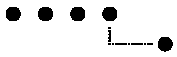
\includegraphics[scale=1.0]{bilder/bfh_de_without_text.pdf}
		\end{textblock}
	}
}

\renewcommand{\chaptermark}[1]{\markboth{\thechapter.  #1}{}}
\renewcommand{\headrulewidth}{0pt}				% no header stripline
\renewcommand{\footrulewidth}{0pt} 				% no bottom stripline

\pagestyle{plain}
%---------------------------------------------------------------------------


% Title Page and Abstract
%---------------------------------------------------------------------------
%
% Project documentation template
% ===========================================================================
% This is part of the document "Project documentation template".
% Authors: brd3
%

\begin{titlepage}


% Red Bar and BFH-Logo absolute placed at (87,10) on A4
% Actually not a realy satisfactory solution but working.
%---------------------------------------------------------------------------
\setlength{\unitlength}{1mm}
\begin{textblock}{210}(-10,-10)
	\begin{picture}(210,32)
		\put(0,0){\color{bfhred}\rule{240mm}{30mm}}
	\end{picture}
\end{textblock}

\begin{textblock}{0}[0,0](84,7)
	
\includegraphics[scale=1.0]{90_bilder/bfh_de_white.pdf}
\end{textblock}

% Titel / Untertitel / Autor:
%---------------------------------------------------------------------------
\begin{flushleft}

\vspace*{4cm}

\fontsize{12pt}{15pt}\selectfont\vspace{0.5em}
Fachbereich Technik und Informatik \\
Herbstsemester 2012

\vspace{2cm}

\fontsize{30pt}{32pt}\selectfont 
\noindent \textbf{Bachelor Thesis - AI Bot f�r Computerspiele} \\
\fontsize{20pt}{22pt}\selectfont 
\noindent \textbf{Ants AI Challenge} \\


\vspace{4cm}
\fontsize{12pt}{15pt}\selectfont
\begin{tabbing}
xxxxxxxxxxxxxxx\=xxxxxxxxxxxxxxxxxxxxxxx \kill
Studierende:	\> Lukas Kuster			\\
							\> Stefan K�ser		\\
																\\
Betreuung:	\> Dr. J�rgen Eckerle	\\
																\\
Experte:	\> Dr. Federico Fl�ckiger	\\
																\\
																\\
Datum:				\> \today					\\
Version:			\> V01.00					\\
\end{tabbing}
\end{flushleft}

%\vspace{6mm}
%\fontsize{12pt}{15pt}\selectfont
%Dieses Dokument dient als Vorlage f�r die Erstellung von Berichten nach den Richtlinien der BFH. Die Vorlage ist in \LaTeX{} %erstellt und unterst�tzt das automatische Erstellen von diversen Verzeichnissen, Literaturangaben, Indexierung und Glossaren. %Dieser kleine Text ist eine Zusammenfassung �ber das vorliegenden Dokument mit einer L�nge von 4 bis 6 Zeilen.

\end{titlepage}

%
% ===========================================================================
% EOF
%

\cleardoubleemptypage
\setcounter{page}{1}
\chapter*{Management Summary}
\label{chap:managementSummary}

Ants AI Challenge ist ein Programmierwettbewerb, bei welchem ein Bot programmiert wird der ein Ameisenvolk steuert. Das Ameisenvolk soll auf einer Map Futtersuchen sowie gegnerische V�lker angreifen und vernichten. Dabei m�ssen Problem wie die Pfadsuche, das Verteilen von Aufgaben sowie das Schwarmverhalten gel�st werden. In unserer Arbeit wollten wir herausfinden was es alles braucht um einen solchen intelligenten Bot zu schreiben und gegen andere Mitspieler anzutreten. Wir konzetrierten uns auf die Aufgabenverteilung sowie die Pfadsuche. Diese Erfahrungen wollen wir f�r die Bachelorarbeit mitnehmen, wo wir an einer aktiven Challenge teilnehmen m�chten oder uns in der f�r dieses Projekt verwendete Challenge vertiefen.

\vspace{5cm}
\begin{tabbing}
xxxxxxxxxxxxxxxxxxxx\=xxxxxxxxxxxxxxxxxxxxxxx \kill
Datum					\> \today \\ \\ \\
Name Vorname	\> Lukas Kuster \\ \\
Unterschrift	\> ......................................................... \\ \\ \\
Name Vorname	\> Stefan K�ser \\ \\
Unterschrift	\> .........................................................
\end{tabbing}


%---------------------------------------------------------------------------

% Table of contents and listings
%---------------------------------------------------------------------------
\tableofcontents
\listoffigures
\listoftables
\cleardoublepage
%---------------------------------------------------------------------------

% Main part:
%---------------------------------------------------------------------------
\pagenumbering{arabic}

\chapter{Einleitung}
\label{chap:einleitung}
Nachdem wir uns im Rahmen des Moduls ''Projekt 2`` (7302) mit der Implementierung eines Bots f�r den Online-Wettbewerb Ants AI-Challenge\footnote{\url{http://www.aichallenge.org}} besch�ftigt hatten, haben wir uns f�r die Bachelorarbeit eine Verbesserung dieses Bots vorgenommen. Ziel des Wettbewerbs ist es jeweils, einen Bot zu programmieren, der durch geschickten Einsatz von KI-Technologien das Spiel m�glichst erfolgreich bestreiten kann.

Im ''Projekt 2`` hatten wir zwar einen Bot implementiert, der alle Aspekte des Spiels einigermassen beherrscht, dazu geh�ren Nahrung sammeln, die Gegend entdecken, H�gel erobern und verteidigen, sowie gegen feindliche Ameisen k�mpfen. Einige dieser F�higkeiten waren aber eher rudiment�r ausgebaut, da wir uns vor allem auf die Pfadsuche konzentriert hatten.

In der Bachelorarbeit ging es nun darum, die taktischen und strategischen Fertigkeiten des Bots auszubauen. Der Schwerpunkt lag auch bei der Bachelorarbeit nicht auf der Optimierung einer Teilaufgabe, sondern auf der Implementierung eines ausgewogenen Bots, der alle Aspekte des Spiels gleichermassen gut beherrscht.

Ein besonderes Augenmerk legten wir dabei auf einen modularen Aufbau des Codes. Nebst einem sauberen objektorientierten Programmdesign spiegelt sich das vor allem in den separaten Modulen ''AITools-Api``, ''Search`` und ''Strategy``, die so generisch implementiert wurden, dass sie mit geringem Aufwand auch in anderen Projekten einsetzbar sind.



\section{Spielbeschrieb}
\label{sec:einleitung.Spielbeschrieb}

\subsection{Der Wettbewerb}
\label{sec:einleitung.Spielbeschrieb.wettbewerb}
Die AI Challenge\footnote{\url{http://www.aichallenge.org}} ist ein internationaler Wettbwerb des University of Waterloo Computer Science Club der im Zeitraum Herbst 2011 bis Januar 2012 zum 3. Mal stattgefunden hat. Das Spiel in dieser 3. Ausf�hrung war ein zugbasiertes Multiplayerspiel in welchem sich Ameisenv�lker gegenseitig bek�mpfen. Ziel in der AI-Challenge ist es, einen Bot zu schreiben, der die gegebenen Aufgaben mit m�glichst intelligenten Algorithmen l�st. Die zu l�senden Aufgaben der Ants AI Challenge sind die Futtersuche, das Explorieren der Karten, das Angreifen von gegnerischen V�lkern und deren Ameisenhaufen sowie dem Sch�tzen des eigenen Ameisenhaufen.

\subsection{Spielregeln}
\label{sec:einleitung.Spielbeschrieb.spielregeln}
Nachfolgend sind die wichtigsten Regeln, die w�hrend dem Spiel ber�cksichtigt werden m�ssen, aufgelistet.
\begin{itemize} 
\item Pro Zug k�nnen alle Ameisen um ein Feld (vertikal oder horizontal) verschoben werden.
\item Pro Zug steht insgesamt eine Rechenzeit von einer Sekunde zur Verf�gung. Es d�rfen keine Threads erstellt werden.
\item Bewegt sich eine Ameise in die 4er Nachbarschaft eines Futterpixels, wird dieses eingesammelt. Beim n�chsten Zug entsteht bei einem Ameisenh�gel eine neue Ameise.
\item Die Landkarte besteht aus passierbaren Landpixeln sowie unpassierbaren Wasserstellen.
\item Ein Gegner wird geschlagen, wenn im Kampfradius der eigenen Ameise mehr eigene Ameisen stehen als gegnerische Ameisen im Kampfradius der Ameise, die angegriffen wird.
\item Ein Gegner ist ausgeschieden wenn alle seine eigenen Ameisenh�gel vom Gegner vernichtet wurden. Pro verlorenem H�gel gib es einen Punkteabzug. Pro feindlichen H�gel, der zerst�rt wird gibt es zwei Bonuspunkte.
\item Steht nach einer definierbaren Zeit (Anzahl Z�ge) kein Sieger fest, wird der Sieger anhand der Punkte ermittelt. 
\end{itemize}
Die ausf�hrlichen Regeln k�nnen auf der Webseite nachgelesen werden: \url{http://aichallenge.org/specification.php}

\subsection{Schnittstelle}
\label{sec:einleitung.Spielbeschrieb.schnittstelle}
Die Spielschnittstelle ist simpel gehalten. Nach jeder Spielrunde erh�lt der Bot das neue Spielfeld mittels String-InputStream, die Spielz�ge gibt der Bot dem Spielcontroller mittels String-OutputStream bekannt. Unser MyBot leitet von der Basis-Klasse Bot\footnote{Die Klasse ist im Code unter ants.bot.Bot.Java auffindbar } ab. Ein Spielzug wird im folgendem Format in den Output-Stream gelegt:
\newline
\newline
o <Zeile> <Spalte> <Richtung>
\newline
\newline
Beispiel:
\begin{verbatim}
o 4 7 W
\end{verbatim}
Die Ameise wird von der Position Zeile 4 und Spalte 7 nach Westen bewegt.
\newline
Der Spielcontroller ist in Python realisiert, der Bot kann aber in allen g�ngigen Programmiersprachen wie Java, Python, C\#, C++ etc. geschrieben werden.

\chapter{Implementation}
\label{chap:implementation}

\section{Modell}
\label{sec:implementation.Model}
F�r die Modellierung habe wir uns auf die n�tigsten Klassen beschr�nkt, um das Modell einfach zu halten. Ein wichtiger Aspekt der Modellierung war dabei die Abbildung des Spiel-Zustands auf State-Klassen, die uns jederzeit Zugriff auf alle bekannten Variablen des Spiels bieten. Einige Informationen k�nnen dabei direkt von der Spiel-Engine �bernommen werden, die meisten Zustandsinformationen werden aber berechnet.

Die Modellierung der Klassen, die Spielelemente repr�sentieren, war etwas einfacher; hier konnten wir auch einzelne Enumerationen u.�. aus dem Beispiel-Bot der AI-Challenge �bernehmen.

\subsection{State-Klassen}
\label{sec:implementation.State}

\begin{figure}[bth]
\centering
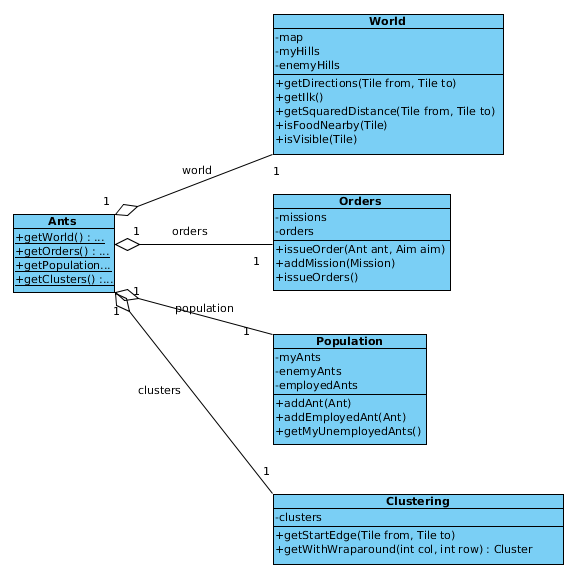
\includegraphics[width=0.7\textwidth]{bilder/State}
\caption{State-Klassen (vereinfacht)}
\label{fig:StateClasses}
\end{figure}

Abbildung \ref{fig:StateClasses} zeigt eine \"{U}bersicht �ber die Zustands-Klassen. F�r das Diagramm wurden lediglich die wichtigsten Methoden und Attribute ber�cksichtigt. Die State-Klassen implementieren alle das Singleton-Pattern.

\subsubsection{Ants}
\label{sec:implementation.State.Ants}
Die Ants Klasse ist die zentrale State-Klasse. Sie bietet auch einfachen Zugriff auf die anderen State-Klassen. Urspr�nglich hatten wir alle Methoden, die mit dem Zugriff auf den Spielzustand zu tun hatten, direkt in der Ants Klasse implementiert, haben aber schnell gemerkt, dass das unhandlich wird. Die Ants Klasse dient jetzt vor allem als Container f�r die anderen State-Klassen und implementiert nur noch einige Methoden, die Zustands�nderungen in verschiedenen Bereichen vornehmen.

\subsubsection{World}
\label{sec:implementation.State.World}
Die World Klasse enth�lt Informationen zur Spielwelt. Hier wird die Karte abgespeichert, in der f�r jede Zelle die aktuell bekannten Informationen festgehalten werden. Das beinhaltet die Sichtbarkeit der Zelle und was die Zelle aktuell enth�lt (Ameise, Nahrung, Wasser, ...). Ausserdem werden Listen gef�hrt, wo sich die eigenen und die bekannten gegnerischen H�gel befinden. Die Klasse bietet Methoden zur Distanzberechnung, gibt Auskunft �ber einzelne Zellen und dar�ber, ob sich Nahrung in der Umgebung einer bestimmten Zelle befindet.

\subsubsection{Orders}
\label{sec:implementation.State.Orders}
In der Orders Klasse wird �ber Befehle und Missionen der einzelnen Ameisen Buch gef�hrt. Die Liste der Befehle wird dabei in jedem Zug geleert und neu bef�llt, w�hrend die Liste der Missionen zug�bergreifend gef�hrt wird. Das zentrale Verwalten der Befehle dient vor allem dazu, sicherzustellen, dass keine widerspr�chlichen Befehle ausgegeben werden (mehrere Befehle f�r eine Ameise, gleiche Ziel-Koordinaten f�r mehrere Ameisen, ...)

\subsubsection{Population}
\label{sec:implementation.State.Population}
Die Population Klasse dient der Verwaltung der eigenen und der gegnerischen Ameisen-V�lker. Hier werden die Ameisen mit ihren aktuellen Aufenthaltsorten festgehalten. Wenn f�r eine Ameise ein Befehl ausgegeben wird, wird die Ameise als besch�ftigt markiert; �ber die Methode \texttt{getMyUnemployedAnts()} kann jederzeit eine Liste der Ameisen abgefragt werden, die f�r den aktuellen Zug noch keine Befehle erhalten haben.

\subsubsection{Clustering}
\label{sec:implementation.State.Clustering}
Die Clustering Klasse dient dem Aufteilen des Spielfeldes in Clusters f�r die HPA*-Suche (s. Abschnitt \ref{subsec:implementation.Pfadsuche.HPAstar}). Hier werden die berechneten Clusters abgelegt, der Zugriff auf sie erfolgt ebenfalls �ber die Clustering Klasse.

\subsection{Spiel-Elemente (Welt)}
\label{sec:implementation.Entities.World}

\begin{figure}[bth]
\centering
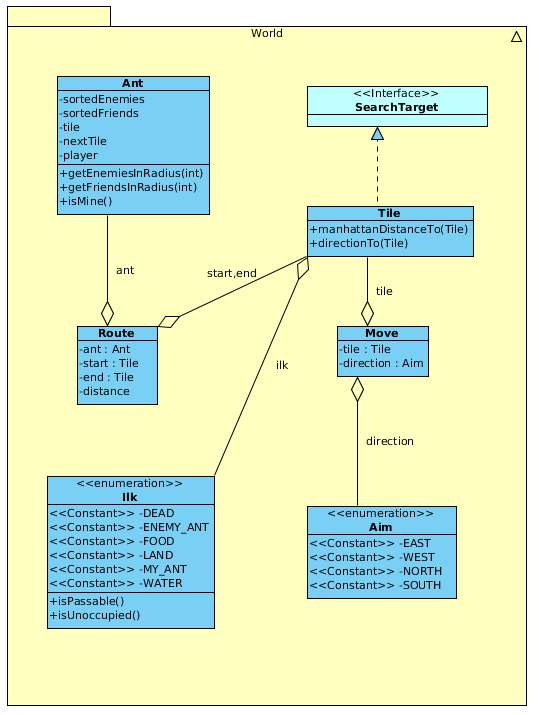
\includegraphics[width=0.7\textwidth]{bilder/Entities_World}
\caption{Spiel-Elemente der Spielwelt (vereinfacht)}
\label{fig:entitiesWorld}
\end{figure}

Abbildung \ref{fig:entitiesWorld} zeigt die wichtigsten Klassen, die die Elemente des Spiels repr�sentieren. Der \"Ubersichtlichkeit wegen wurden nur die wichtigsten Attribute und Operationen in das Diagramm aufgenommen.

\subsubsection{Ant}
\label{sec:implementation.Entities.Ant}
Eine Ant geh�rt immer zu einem Spieler; �ber die Methode isMine() k�nnen unsere eigenen Ameisen identifiziert werden. 
Eine Ameise weiss jeweils, in welcher Zelle sie steht. Das Feld nextTile dient der Verfolgung einer Ameise �ber mehrere Z�ge -- das Feld wird jeweils aktualisiert, wenn der Ameise ein Befehl ausgegeben wird; im n�chsten Zug k�nnen wir dann pr�fen, ob die Ameise den Befehl korrekt ausf�hren konnte. Eine Ameise kennt auch die anderen Ameisen in ihrer Umgebung: �ber die Methoden getEnemies/FriendsInRadius() k�nnen alle bekannten Freunde und Feinde in einem bestimmten Radius ermittelt werden.

\subsubsection{Tile}
\label{sec:implementation.Entities.Tile}
Das Tile repr�sentiert eine Zelle des Spielfelds. Es implementiert das SearchTarget Interface (s. \ref{sec:implementation.Entities.SearchTarget}). Es bietet zudem Methoden f�r die einfache Distanzberechnung, sowie f�r das Bestimmen der Richtungen, in die ein anderes Tile liegt.

\subsubsection{Route}
\label{sec:implementation.Entities.Route}
Eine Route repr�sentiert eine einfache Start-Ziel Verbindung. Sie h�lt f�r eine Ameise die Luftliniendistanz zu einem bestimmten Ziel-Feld fest.

\subsubsection{Move}
\label{sec:implementation.Entities.Move}
Ein Move entspricht einem Zug einer Ameise. F�r ein bestimmtes Tile wird angegeben, in welche Richtung sich die Ameise bewegen soll.

\subsubsection{Ilk}
\label{sec:implementation.Entities.Ilk}
Ilk ist der Typ einer Zelle. Der Ilk einer Tile-Instanz gibt an, was sich gerade in der Zelle befindet. Dies kann eine Gel�nde-Typ sein, wenn die Zelle ansonsten leer ist, oder es kann eine Ameise, Nahrung, oder eine H�gel sein. Die Ilk-Enumeration bietet Hilfsmethoden, um festzustellen, ob eine Zelle passierbar oder besetzt ist.

\subsubsection{Aim}
\label{sec:implementation.Entities.Aim}
Aim ist einfach eine Repr�sentation einer Himmelsrichtung

\subsection{Spiel-Elemente (Suche)}
\label{sec:implementation.Entities.Search}

\begin{figure}[bth]
\centering
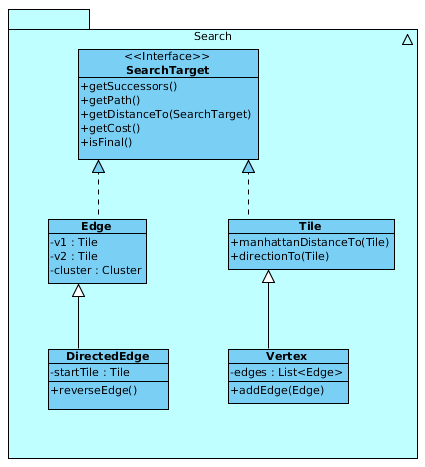
\includegraphics[width=0.7\textwidth]{bilder/Entities_Search}
\caption{Spiel-Elemente f�r die Suche (vereinfacht)}
\label{fig:entitiesSearch}
\end{figure}

Abbildung \ref{fig:entitiesSearch} zeigt die wichtigsten Klassen, die f�r die Pfadsuche verwendet werden. Der \"Ubersichtlichkeit wegen wurden nur die wichtigsten Attribute und Operationen in das Diagramm aufgenommen.

\subsubsection{SearchTarget}
\label{sec:implementation.Entities.SearchTarget}

\subsection{Tasks}
\label{sec:implementation.Tasks}

\begin{figure}[bth]
\centering
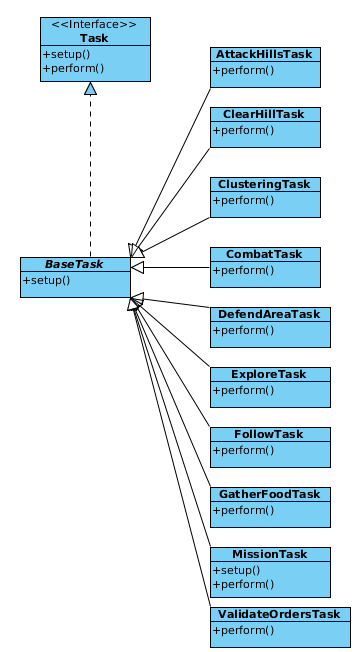
\includegraphics[width=0.5\textwidth]{bilder/Tasks}
\caption{Tasks}
\label{fig:tasks}
\end{figure}

Die Tasks bzw. Aufgaben des Bots wurden in eigenen Klassen implementiert. Das Interface Task\footnote{Das Interface ist im Code unter ants.tasks.Bot.Java auffindbar.} definiert eine setup()-Methode welche den Task initiert, sowie eine perform()-Methode welche den Task ausf�hrt. Im Programm werden die Tasks nach deren Wichtigkeit ausgef�hrt, was auch der nachfolgenden Reihenfolge entspricht. Jedem Task stehen nur die unbesch�ftigten Ameisen zur Verf�gung, d.h. jene welchen noch keine Aufgabe zugeteilt wurde.

\subsubsection{MissionTasks}
\label{subsec:implementation.Tasks.MissionTask}
Dieser Task pr�ft alle akutellen Missionen auf deren G�ltigkeit, beispielsweise ob die Ameise der Mission den letzten Zug �berlebt hat und die Mission weiterf�hren kann. Falls g�ltig, wird der n�chste Schritt der Mission ausgef�hrt.

\subsubsection{GatherFoodTask}
\label{subsec:implementation.Tasks.GatherFoodTask}
F�r jedes Food-Tile wird in einem definierbaren Radius r die n�chsten Ameisen bestimmt. Danach wird aufsteigend der Luftliniendistanz versucht mit dem Pfadsuchalgorithmus SIMPLE (s. Abschnitt \ref{subsec:implementation.Pfadsuche.Simple}) oder falls dieser kein Pfad gefunden hat mit A* eine passierbare Route gesucht. Wenn ein Pfad existiert, kann mit der Ameise und dem Food-Tile eine GatherFoodMission erstellt werden, welche die Ameise zum Food-Tile f�hrt. Zu jedem Food-Tile wird immer nur eine Ameise geschickt.

\subsubsection{AttackHillsTask}
\label{subsec:implementation.Tasks.AttackHillsTask}
Sobald gegnerische Ameisenhaufen sichtbar sind, sollen diese angegriffen werden. Falls dieser, wie bereits erw�ht, zerst�rt wird, werden  zwei Bonuspunkten gutgeschrieben. Die Kriterien, dass eine Pfad zum gegnerischen Haufen gesucht wird, sind die selben wie beim GatherFoodTask, ausser dass mehrere Ameisen das Ziel angreifen k�nnen. Es wird ein AttackHillMission erstellt.

\subsubsection{CombatTask}
\label{subsec:implementation.Tasks.CombatTask}
Beim Angriffstask wird berechnet ob wir in einem Kampfgebiet (viewRadius2) die �berhand, d.h mehr Ameisen platziert haben. Falls ja wird die gegnerische Ameise angegriffen.

\subsubsection{DefendAreaTask}
\label{subsec:implementation.Tasks.DefendAreaTask}
Dieser Task w�re vogesehen um eine Region wie zum Beispiel der eigene Ameisenh�gel zu sch�tzen. Dieser Task wurde mit im Zuge dieser Arbeit nicht implementiert.

\subsubsection{ExploreTask}
\label{subsec:implementation.Tasks.ExploreTask}
F�r alle noch unbesch�ftigten Ameisen wird mittels ManhattanDistance der n�chste Ort gesucht, der noch nicht sichtbar, also unerforscht ist. Falls ein Pfad mittels Pfadsuchalgorithmus gefunden wird, wird eine ExplorerMission (s. Abschnitt \ref{sec:implementation.Missionen}) erstellt. Die Ameise wird den gefundenen Pfad in den n�chsten Spielz�gen ablaufen.

\subsubsection{FollowTask}
\label{subsec:implementation.Tasks.FollowTask}
Der FollowTask ist f�r Ameisen angedacht welche aktuell keine Aufgabe haben. Diese Ameisen sollen einer nahe gelegenen, besch�ftigten Ameise folgen, damit diese nicht alleine unterwegs ist.

\subsubsection{ClearHillTask}
\label{subsec:implementation.Tasks.ClearHillTask}
Dieser Task bewegt alle Ameisen, welche neu aus unserem H�gel \"schl�pfen\" vom H�gel weg. So werden nachfolgende Ameisen nicht durch diese blockiert.

\subsubsection{ClusteringTask}
\label{subsec:implementation.Tasks.ClusteringTask}
Der ClusteringTask wird als Vorbereitung f�r den HPA* Algorithmus verwendet. Hier wird f�r alle sichtbaren Kartenregionen ein Clustering vorgenommen. Das Clustering wird im Kapitel \ref{subsec:implementation.Pfadsuche.HPAstar} im Detail beschreiben.

\subsection{Missionen}
\label{sec:implementation.Missionen}
Eine Mission dauert �ber meherer Spielz�ge. Die meisten Missionen (GatherFoodMission, ExploreMission, AttackHillMission, AttackAntMission) sind Pfadmissionen\footnote{Die abstrakte Klasse PathMission ist im Code unter ants.missions.PathMission.java auffindbar.} bei welchen die Ameise einem vorgegebenen Pfad, der bereits beim Erstellen der Mission berechnet wurde, folgt. Je nach spezifischer Mission sind aber die Abbruchbedingungen anders. Zum Beispiel die GatherFoodMission ist nur solange g�ltig wie das Futter noch nicht von einer anderen Ameise eingesammelt wurde.


\section{Bot}
\label{sec:implementation.Bot}


\begin{figure}[bth]
\centering
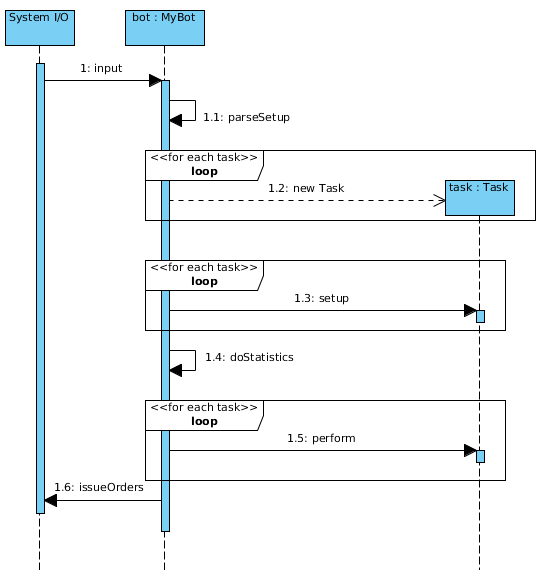
\includegraphics[width=0.9\textwidth]{bilder/FirstTurn}
\caption{Ablauf des ersten Zugs des Spiels}
\label{fig:firstTurn}
\end{figure}

\begin{figure}[bth]
\centering
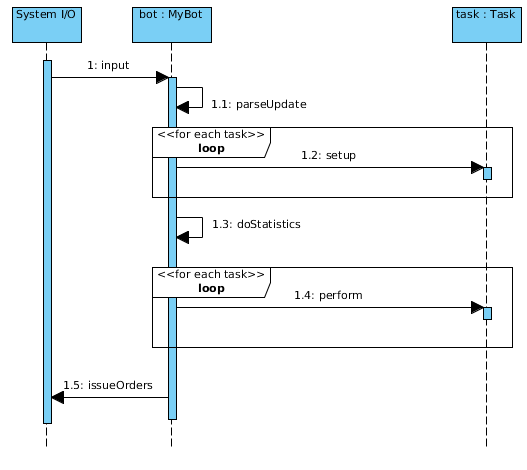
\includegraphics[width=0.9\textwidth]{bilder/Turn}
\caption{Ablauf der weiteren Z�ge des Spiels}
\label{fig:turn}
\end{figure}


\section{Pfadsuche}
\label{sec:implementation.Pfadsuche}
Wir haben drei m�gliche Pfadalgorithmen in unserem Code eingebaut. Via PathFinder-Klasse kann f�r die Pfadsuche der Alogrithmus ausgew�hlt werden.


\subsection{Simple Algorthmus}
\label{subsec:implementation.Pfadsuche.Simple}

Der Simple Algorithmus versucht das Ziel zu erreichen indem er zuerst die eine, dann die andere Achse abl�uft. Sobald ein Hindernis in den Weg kommt bricht der Algorithmus ab. Im folgenden Beispiel sucht der Alogrithmus den Vertikal-Horizontal Pfad. Da dieser Pfad wegen dem Wasserhindernis (blau) nicht ans Ziel f�hrt, wird via Horizontal-Vertikal Pfad gesucht. Hier wird ein Pfad gefunden. Dieser Algorithmus ist, wie der Name bereits aussagt, sehr einfach aufgebaut und kostet wenig Rechenzeit. Daf�r kann er keinen Hindernissen ausweichen.

\begin{figure}
\centering
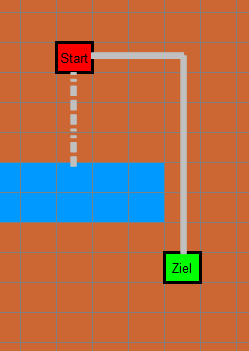
\includegraphics[height=50mm]{bilder/simplepath}
\caption{Simple-Path Algorithmus}
\label{fig:SimplePath}
\end{figure}

\subsection{A* Algorthmus}
\label{subsec:implementation.Pfadsuche.Astar}
Beim A* Algorithmus wird f�r jeden expandierten Knoten einen heuristischen Wert f(x) f�r gesamte Pfadl�nge berechnet. f(x) besteht aus einem Teil g(x) welches die effektiven Kosten vom Startknoten zum aktuellen Knoten berechnet. Der andere Teil h(x) ist ein heuristischer Wert der die Pfadkosten welche bis zum Zielknoten approximiert. Dieser Wert muss die effektiven Kosten zum Ziel immer untersch�tzen. Dies ist in unserem Spiel dadurch gegeben, dass sich die Ameisen nicht diagonal bewegen k�nnen, wir aber f�r den heuristischen Wert die Luftlinie zum Ziel verwenden. Die Pfadsuche wird immer bei dem Knoten fortgesetzt welcher die kleinsten Kosten f(x) hat.

\begin{figure}
\centering
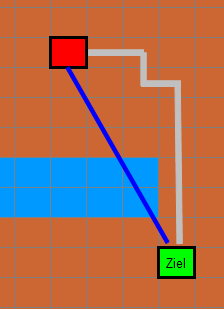
\includegraphics[height=50mm]{bilder/heuristicAstar.png}
\caption{Heuristische Kosten (blau), Effektive Kosten (grau)}
\label{fig:heuristicAstar}
\end{figure}

Das Bild zeigt den effektiven Pfad (grau) vom expandierenden roten Knoten mit den minimalen Kosten von 10 Pixel. Die Luftlinie (blau) als heurstischer Wert hat aber nur eine L�nge von 7.6 Pixel. Damit erf�llt unsere Implementation die Anforderungen des Algorithmus.

Dieser Algorithmus wird in unserem Code f�r eine Pfadsuche �ber alle Pixel (jedes Pixel ist ein Node) verwendet. Der gleiche Code wir aber auch f�r die Pfadsuche mit dem Pfadnetz des HPA* verwendet.

\subsection{HPA* Algorthmus}
\label{subsec:implementation.Pfadsuche.HPAstar}

Eine Pfadsuche A* �beralle Pixel ist sehr teuer, da es viel Pfade gibt, die zum Teil nur ein Pixel nebeneinander liegen. Es werden bis zum Schluss verschiedenen Pfaden nachgegangen. Abhilfe zu dieser sehr feinmaschigen Pfadsuche bietet der Hierarcical Pathfinding A* bei welchem im sogenanten Clustering �ber mehrere Pixel verlaufende Kanten und Knoten berechnet werden.

\paragraph[Clustering]{Clustering}
Das Clustering wird w�hrend dem ClusteringTask ausgef�hrt, Dabei wird die Landkarte in sogenannte Clusters unterteilt. Auf dem Bild \ref{fig.clusteredMap} wurde die Karte in 16 Clusters aufgeteilt. 

\begin{figure}
\centering
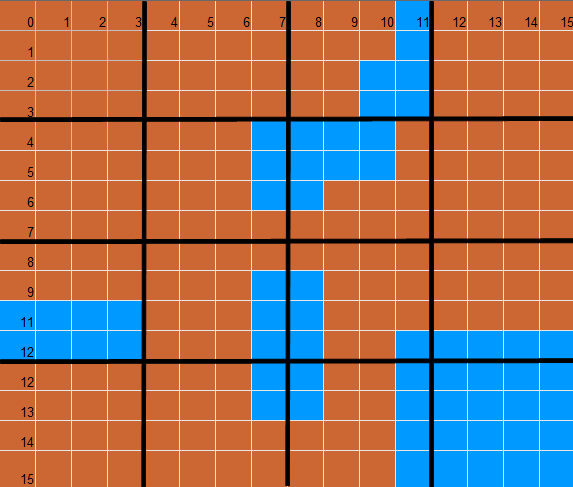
\includegraphics[height=50mm]{bilder/clusteredMap.png}
\caption{Clustereinteilung auf der Landkarte. Clustergr�sse 4x4, Landkarte 16x16}
\label{fig.clusteredMap}
\end{figure}

Danach wird f�r jeden Cluster und ein Nachbar aus der vierer Nachbarschaft die Verbindungskanten berechnet. Dies kann nat�rlich nur f�r Clusters gemacht werden die auf einem sichtbaren Teil der Landkarte liegen, was zu Begin des Spiel nicht gegeben ist. Deshalb wird der ClusteringTask in jedem Spielzug aufgerufen, in der Hoffnung ein Cluster komplett verbinden zu k�nnen. Sobald eine beliebige Seite eines Clusters berechnet ist, wird diese Aussenkante im Cluster und dem anleigenden Nachbar gespeichert und nicht mehr neu berechnet.

\begin{figure}
\centering
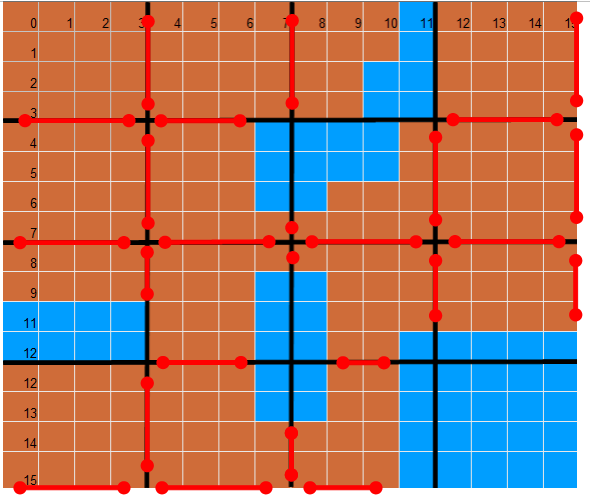
\includegraphics[height=50mm]{bilder/clusteredMap2.png}
\caption{Die Kanten jedes Clusters wurden berechnet}
\label{fig.clusteredMap2}
\end{figure}

Sobald ein Cluster zwei oder mehrere Aussenkanten kennt berechnet er die Innenkanten mit A* welche die Knoten der Aussenkanten verbindet. Dies ergibt nun ein Pfadnetz �ber die Gesamtkarte.
\newline
Nun wird ein Pfad vom Pixel (0,9) nach (14,9) gesucht. Zuerst wird eruiert in welchem Cluster sich das Start- bzw Zielpixel befindet. Danach wird in dem gefundenen Cluster ein Weg zu einem beliebigen Knoten auf der Clusterseite gesucht. Sind diese Knoten erreicht kann nun das vorberechnete Pfadnetz mittels bereits beschrieben A* Algroithmus verwendet werden um die beiden Knoten auf dem k�rzesten m�glichen Pfad zu verbinden.\footnote{Der gefundene Pfad k�nnte mittels Pathsmoothing verk�rzt werden. Dies wurde aber in unserer Arbeit nicht implementiert.}

TODO Beispielbild

\section{JavaScript Addon f�r HMTL-Gameviewer}
\label{sec:implementation.Addon}
Das Codepaket welches von den Challengeersteller mitgeliefert wird bietet bereits eine hilfreiche 2D-Visualisierung des Spiels mit welchem das Spielgeschehen mitverfolgt werden kann. Die Visualisierung wurde mit HMTL und Javascript implementiert. Leider ist es nicht m�glich zus�tzliche Informationen auf die Seite zu projizieren. Deshalb haben wir den Viewer mit einer solchen Funktion erweitert. Mit der Codezeile Logger.liveInfo(...) kann eine Zusatzinformation geschrieben werden. Es muss definiert werden mit welchem Zug und wo auf dem Spielfeld die Infomation angezeigt werden soll. Im Beispiel wird an der Position der Ameise ausgegeben welchen Task die Ameise hat.
\begin{verbatim}
Logger.liveInfo(Ants.getAnts().getTurn(), ant.getTile(), "Task: %s ant: %s", issuer, ant.getTile());
\end{verbatim}
Auf der Karte wird ein einfaches aber praktisches Popup mit den geschriebenen Informationen angezeigt. Dank solchen Zusatzinfomrationen muss nicht m�hsam im Log nach geschaut werden, welcher Ameise wann und wo welcher Task zugeordnet ist.

\begin{figure}
\centering
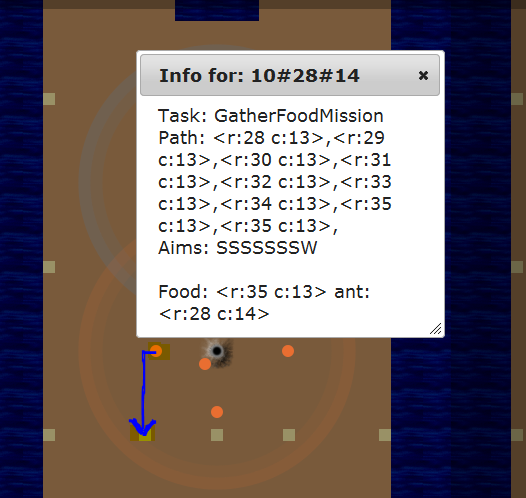
\includegraphics[height=70mm]{bilder/javascriptAddon.png}
\caption{Das Popup zeigt dei Aufgabe und den Pfad (blau), welcher die Ameise ablaufen wird.}
\label{fig.javascriptAddon}
\end{figure}

Das angezeigte Popup zeigt welchen Task (GatherFoodTask) die Ameise hat, wo sie sich befindet <r:28 c:14>, welches Futterpixel angesteuert wird <r:35 c:13> und welchen Pfad dazu berechnet wurde. 
\chapter{R�ckblick}
\label{chap:rueckblick}

\section{Resultate}
\label{sec:rueckblick_resultate}
Wir haben mit dieser Arbeit einen guten Einblick in die Programmierung von Bots erhalten. Uns ist bewusst geworden, dass viele Aspekte zusammenspielen m�ssen, damit sich die einzelnen Ameisen intelligent verhalten. Da die Spielschnittstelle einfach gehalten und im Web gut dokumentiert ist kamen wir relativ schnell zu einem sichtbaren Resultat, indem bereits erste Spiele verfolgt werden konnten. Mit einem sauberen Aufbau des Programmcodes konnten wir die Aufgaben einfach gliedern und haben einen guten Grundstein gelegt, falls wir dieses Projekt als Bachelorarbeit weiterverfolgen. Dank den eingesetzten Pfadsuchalgorithmen konnten wir die Rechenzeit verringern und haben so w�hrend einem Zug genug Zeit um weitere Berechnungen zu machen. 

\section{Herausforderungen}
\label{sec:spielbeschrieb_herausforderungen}
Beim Suchen eines Programmierfehlers musste das Logfile durchforstet werden, was sich als eine aufw�ndige und zeitraubende Arbeit herausstellte. Dadurch sind wir auch auf die Idee des Javascript Addon gekommen. Zu Beginn der Arbeit wurde die zur Verf�gung stehende Zeit eines Zuges rasch aufgebraucht, da wir keinen schlauen Algorithmus f�r die Pfadsuche verwendeten; dies konnte mit A* und HPA* behoben werden.

\section{Ziele f�r Bachelorarbeit}
\label{sec:spielbeschrieb_zieleBachelorarbeit}
Im Projekt 2 haben wir uns vor allem auf die Pfadsuche konzentriert. Die Spiele-Entwicklung beinhaltet aber auch Strategie und Taktik. Dies konnte noch nicht angeschaut werden und wird sicher ein Teil der Bachelorarbeit sein. Die Ameisen sollten sich in einem Schwarm fortbewegen, damit sie im Kampf st�rker sind. Dies zu implementieren w�re eine interessante Herausforderung in einem Kerngebiet der K�nstlichen Intelligenz.
Weiter kann gepr�ft werden, ob ein supervised oder ein unsupervised Learning eingebaut werden kann.

Die Organisatoren der AI Challenge sind allerdings bereits dabei, die n�chste Challenge zu planen. Falls sich das n�chste Spiel als geeignet f�r eine Bachelorarbeit erweist, w�rden wir es bevorzugen, an dieser Challenge teilzunehmen, da wir uns so auch direkter mit den anderen Teilnehmern messen k�nnten.


% Attachment:
%---------------------------------------------------------------------------
\appendix
\settocdepth{section}
\chapter{Beliebiger Anhang}
\label{chap:bel_anhang}

Phasellus eget velit massa, sed faucibus nisi. Etiam tincidunt libero viverra lorem bibendum ut rutrum nisi volutpat. Donec non quam vitae lacus egestas suscipit at eu nisi. Maecenas non orci risus, at egestas tellus. Vivamus quis est pretium mauris fermentum consectetur. Cras non dolor vitae nulla molestie facilisis. Aliquam euismod nisl eget risus pretium non suscipit nulla feugiat. Nam in tortor sapien. Nam lectus nibh, laoreet eu ultrices nec, consequat nec sem. Nulla leo turpis, suscipit in vulputate a, dapibus molestie quam. Vestibulum pretium, purus sed suscipit tempus, turpis purus fermentum diam, id cursus enim mi a tortor. Proin imperdiet varius pellentesque. Nam congue, enim sit amet iaculis venenatis, dui neque ornare purus, laoreet porttitor nunc justo vel velit. Suspendisse potenti. Nulla facilisi.

\chapter{Weiterer Anhang}
\label{chap:anhang_B}

\section{Test 1}
Phasellus eget velit massa, sed faucibus nisi. Etiam tincidunt libero viverra lorem bibendum ut rutrum nisi volutpat. Donec non quam vitae lacus egestas suscipit at eu nisi. Maecenas non orci risus, at egestas tellus. Vivamus quis est pretium mauris fermentum consectetur. Cras non dolor vitae nulla molestie facilisis. Aliquam euismod nisl eget risus pretium non suscipit nulla feugiat. Nam in tortor sapien. 

\subsection{Umfeld}
Nam lectus nibh, laoreet eu ultrices nec, consequat nec sem. Nulla leo turpis, suscipit in vulputate a, dapibus molestie quam. Vestibulum pretium, purus sed suscipit tempus, turpis purus fermentum diam, id cursus enim mi a tortor. Proin imperdiet varius pellentesque. Nam congue, enim sit amet iaculis venenatis, dui neque ornare purus, laoreet porttitor nunc justo vel velit. Suspendisse potenti. Nulla facilisi.

%---------------------------------------------------------------------------

% Glossary
%---------------------------------------------------------------------------
\cleardoublepage
\phantomsection 
\addcontentsline{toc}{chapter}{Glossar}
\renewcommand{\glossaryname}{Glossar}
\printglossary
%---------------------------------------------------------------------------

% Bibliography
%---------------------------------------------------------------------------
\cleardoublepage
\phantomsection 
\addcontentsline{toc}{chapter}{Literaturverzeichnis}
\bibliographystyle{IEEEtranS}
\bibliography{datenbanken/bibliography}{}
%---------------------------------------------------------------------------

% Index
%---------------------------------------------------------------------------
\cleardoublepage
\phantomsection 
\addcontentsline{toc}{chapter}{Stichwortverzeichnis}
\renewcommand{\indexname}{Stichwortverzeichnis}
\printindex
%---------------------------------------------------------------------------

%---------------------------------------------------------------------------
\end{document}

